\chapter{Instrukcja użytkownika}
\label{chap:instrukcja-uzytkownika}
Ze względu na dwie ścieżki użytkowania aplikacji, instrukcja użytkownika została podzielona na dwie sekcje: dla studentów oraz dla biznesu.
\section{Student - przykład tworzenia projektu}
Użytkownik student najpierw musi się zarejestrować w aplikacji, ekran jest pokazany na rysunku \ref{fig:rejestracja_landing_student}a.
Następnie użytkownik zostaje przekierowany do strony głównej aplikacji skąd może założyć nowe projekty, przedstawionego na rysunku \ref{fig:rejestracja_landing_student}b.
\begin{figure}[!htb]
    \centering
    \begin{tabular}{ll}
    a) & 
    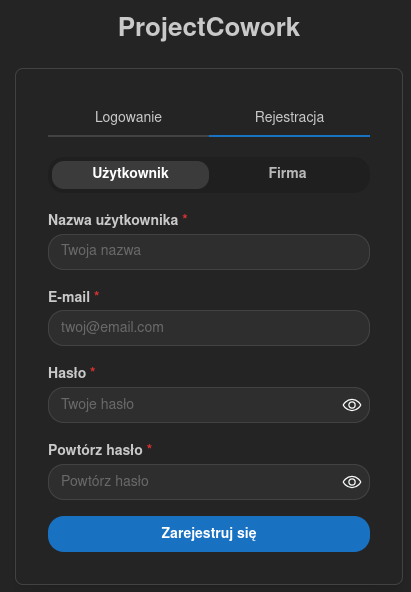
\includegraphics[scale=0.5]{rysB/start_student.png} \\
    b) &
    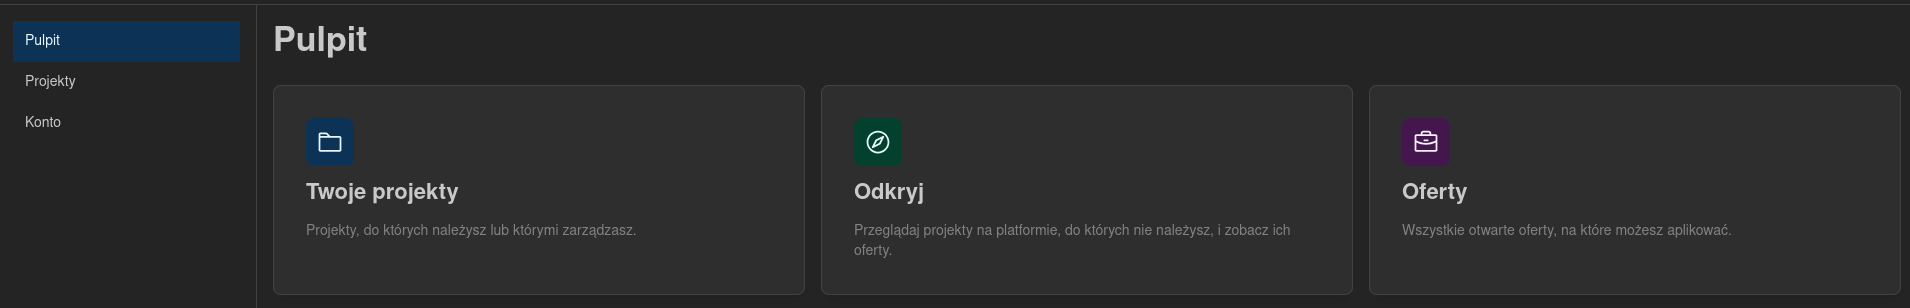
\includegraphics[scale=0.33]{rysB/strona_g_student.png}
    \end{tabular}
    \caption{a) Ekran rejestracji studenta, b) strona główna studenta}
    \label{fig:rejestracja_landing_student}
\end{figure}

Po przejściu do strony moje projekty, użytkownik może utworzyć projekt, co zostało pokazane na rysunku \ref{fig:dodawanie_student}.
\begin{figure}[!htb]
    \centering
    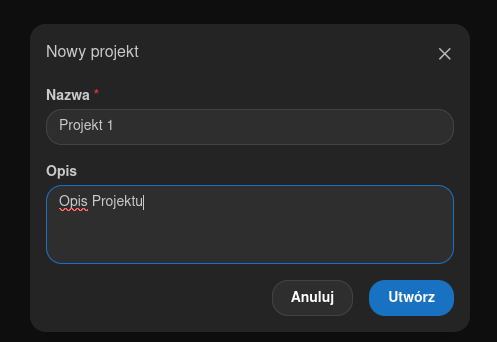
\includegraphics[scale=0.5]{rysB/nowy_projekt_student.png}
    \caption{ekran dodawania projektu}
    \label{fig:dodawanie_student}
\end{figure}
\newpage
Po dodaniu projektu, użytkownik go zobaczy i może wejśc w jego szczegóły. Szczegóły mają swoje sekcje na stronie projektu, przedstawione na rysunkach \ref{fig:projekt}
\begin{figure}[!htb]
    \centering
    \begin{tabular}{ll}
        a) & 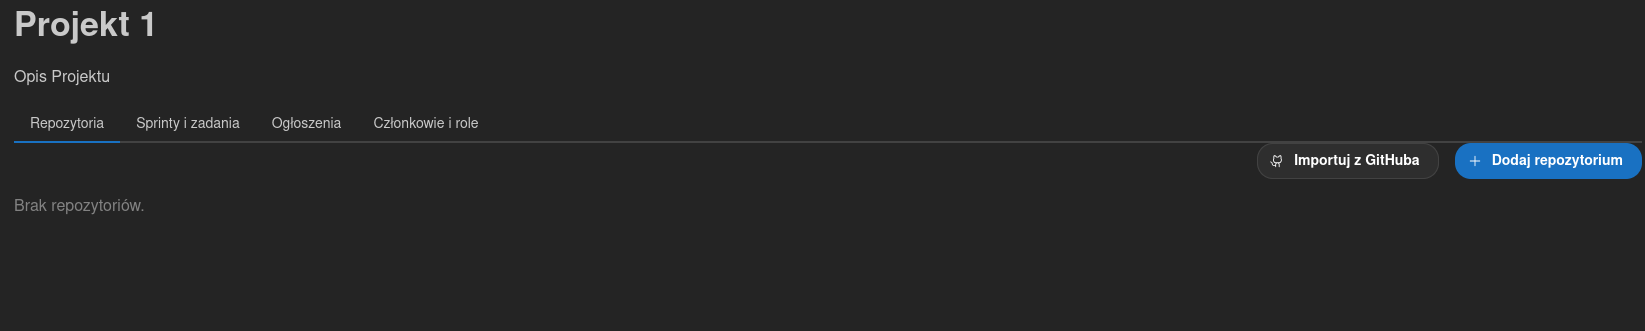
\includegraphics[scale=0.35]{rysB/panel_projekt_student.png} \\
        b) & 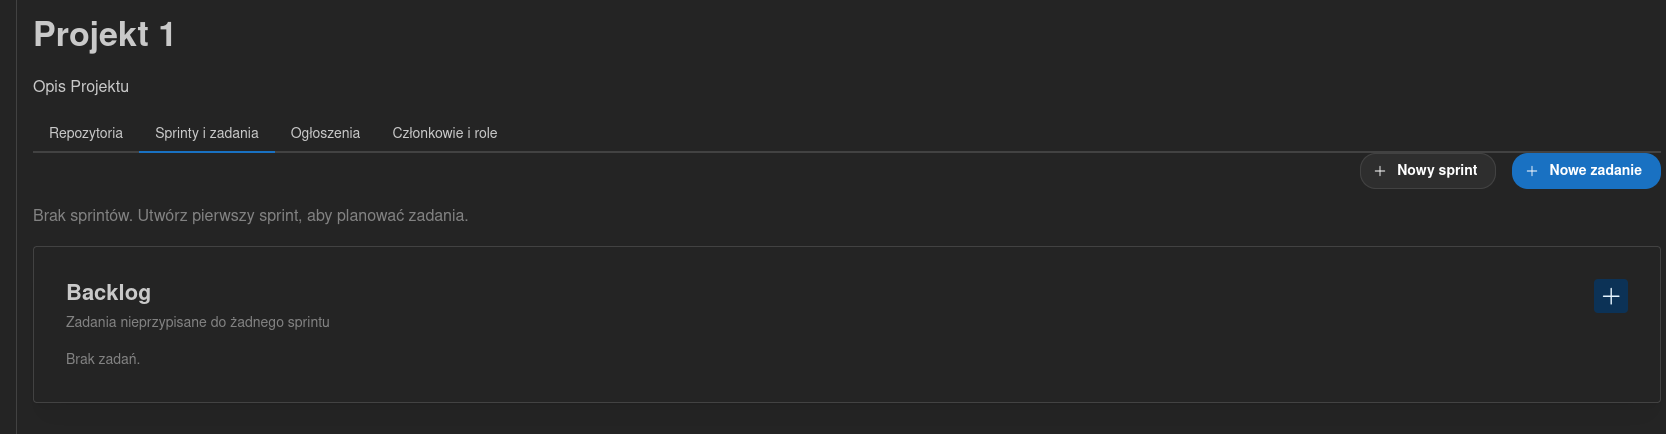
\includegraphics[scale=0.35]{rysB/panel_sprinty.png} \\
        c) & 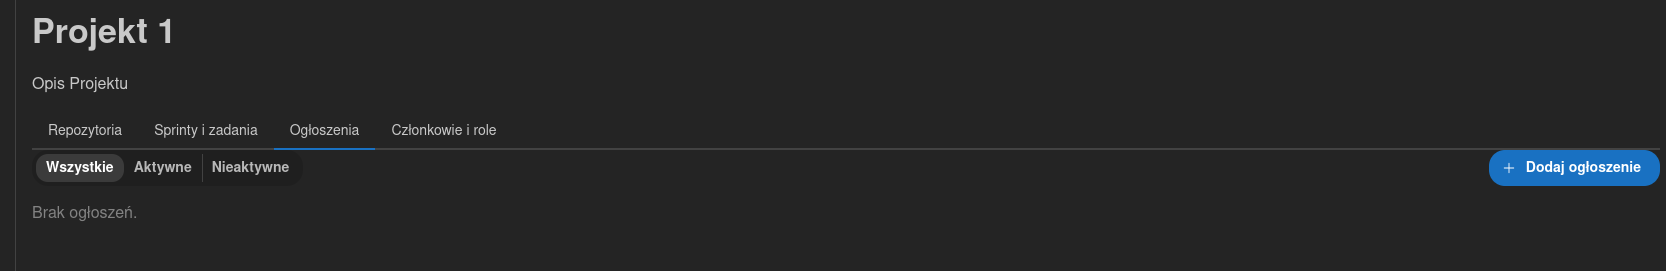
\includegraphics[scale=0.35]{rysB/projekt_ogłoszenia.png} \\
        d) & 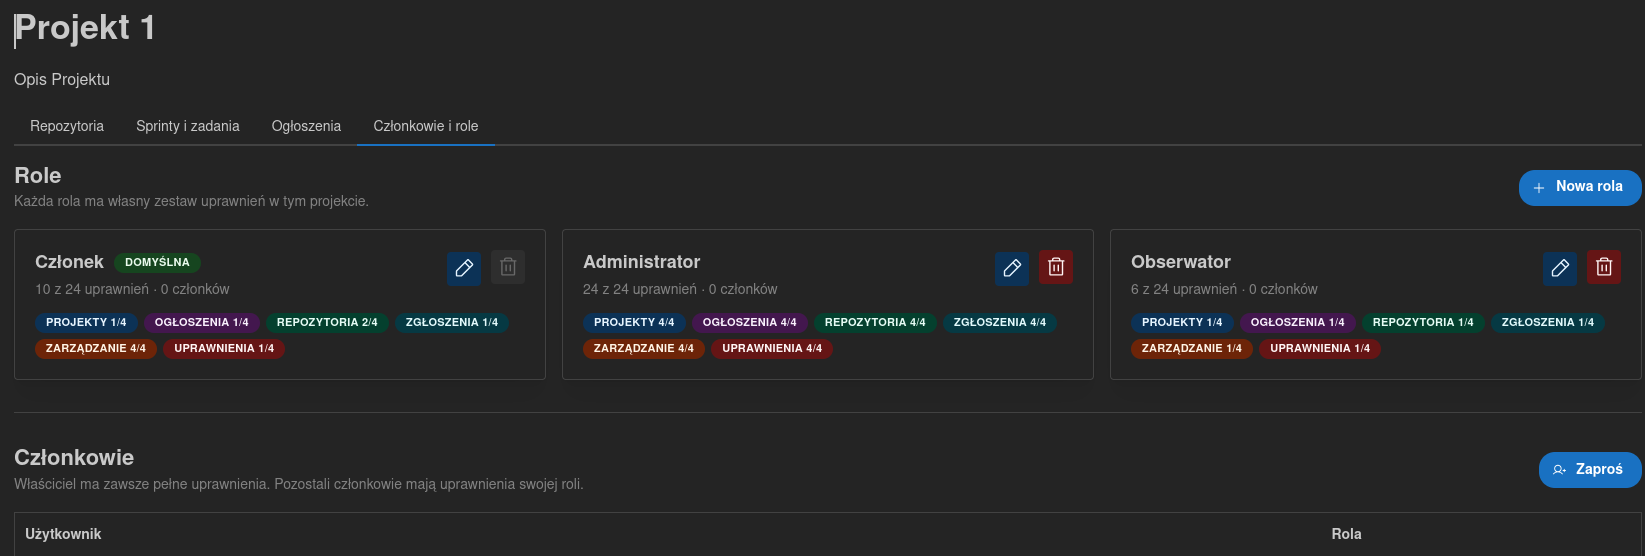
\includegraphics[scale=0.35]{rysB/projekt_czlonki.png}
    \end{tabular}
    \caption{a) panel repozytoriów projektu b) panel sprintów i zadań projektu c) panel ogłoszeń projektu d) panel członków projektu}
    \label{fig:projekt}
\end{figure} \\ \\
Zgodnie z kolejnością, użytkownik może zarządzić repozytoriami - może na przykład dodać nowe i wejść w jego szczegóły, może utworzyć sprint i zadania w nim, może
dodawać ogłoszenia na zapotrzebowanie do projektu lub zarządzać członkami projektu. Interfejs został zaprojektowany by być jak najprostszym i intuicyjnym dla użytkownika.
Podany został najprostszy przykład tego jak utworzyć projekt w systemie.
\section{Biznes}
Tak, jak wyżej, Użytkownik biznesowy najpierw musi się zarejestrować w aplikacji, ekran jest pokazany na rysunku \ref{fig:rejestracja_biznes}.
\begin{figure}[!htb]
    \centering
    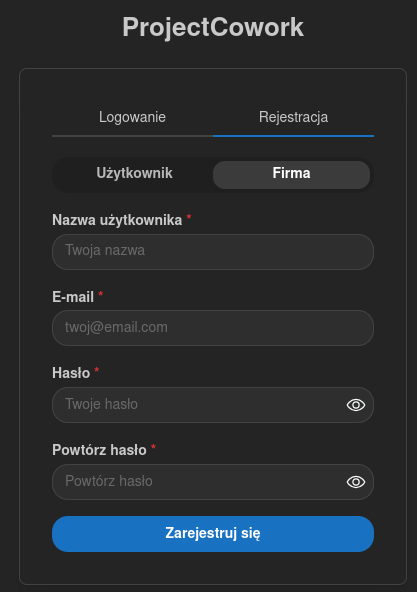
\includegraphics[scale=0.5]{rysB/start_biznes.png}
    \caption{Ekran rejestracji biznesu}
    \label{fig:rejestracja_biznes}
\end{figure} \\
Po zarejestrowaniu się, użytkownik zostanie zautoryzowany i będzie miał dostęp do aplikacji. Zostanie od razu przekierowany na stronę główną pokazaną na rysunku \ref{fig:landing_biznes}
\begin{figure}[!htb]
    \centering
    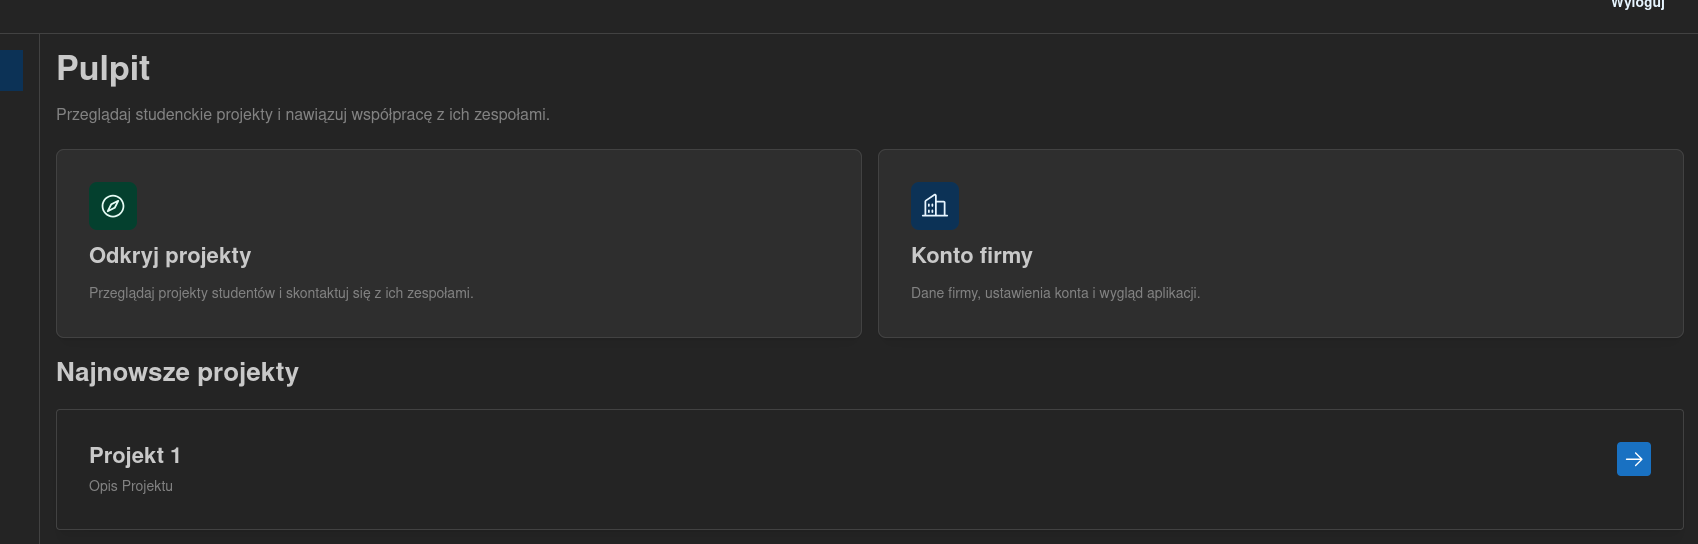
\includegraphics[scale=0.35]{rysB/glowna_firma.png}
    \caption{Strona główna biznesu}
    \label{fig:landing_biznes}
\end{figure}
\newpage
Na niej użytkownik może zobaczyć najnowsze projekty na platformie i może przejść do ogólnego widoku projektów lub ustawień swojego konta pokazanych na rysunku \ref{fig:firma}a i \ref{fig:firma}b.
\begin{figure}[!htb]
    \begin{tabular}{ll}
        a) & 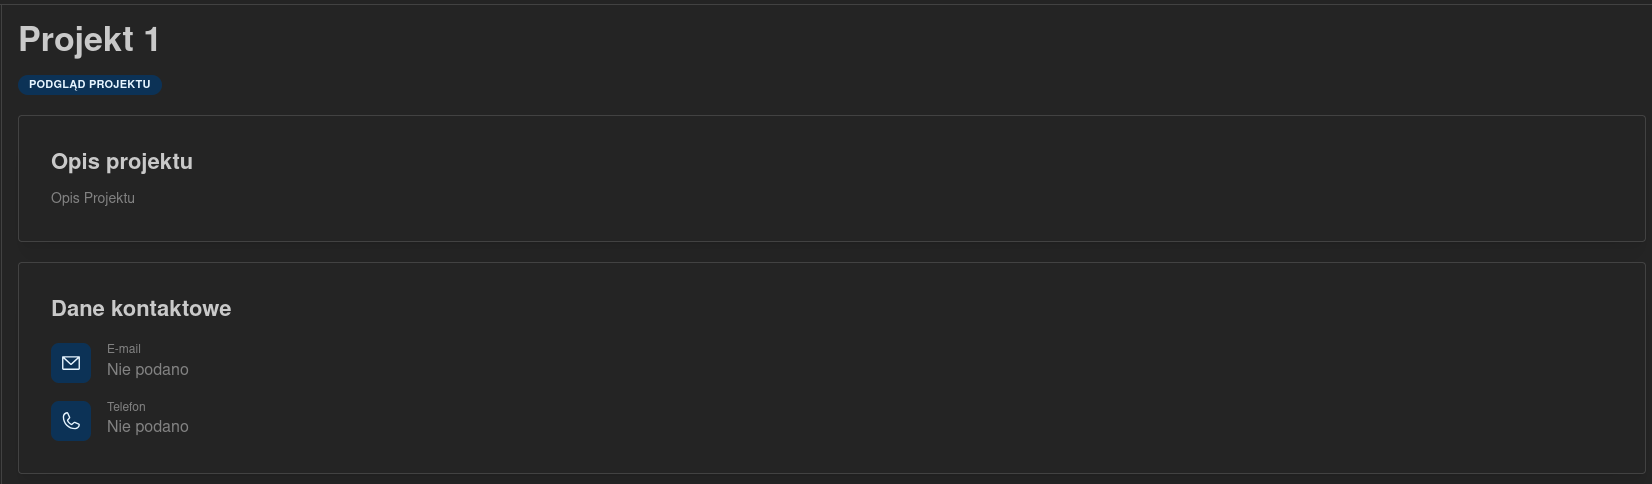
\includegraphics[scale=0.3]{rysB/panel_projekt_firma.png} \\
        b) & 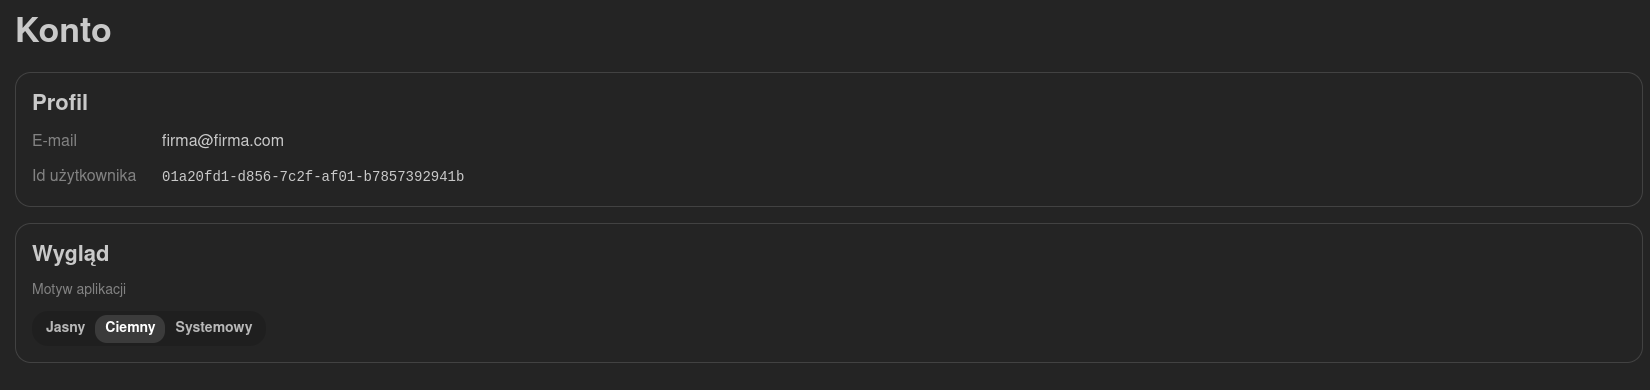
\includegraphics[scale=0.3]{rysB/panel_ustawien_firma.png}
    \end{tabular}
    \caption{a) panel projektów b) panel ustawień konta biznesowego}
    \label{fig:firma}
\end{figure} \\
Użytkownik biznesowy może z panelu projektu skontaktować się z twórcami z poziomu danych kontaktowych. Natomiast z poziomu ustawień może zmieniać ustawienia systemu.
Panel ten jest ograniczony i maksymalnie uproszczony.